\subsection{Rediseño del 'Arbol de An'alisis}

Para solucionar las limitaciones presentadas nos propusimos rediseñar el 'arbol de an'alisis.
El primer cambio que realizamos es la implementaci'on de \emph{heterogeneidad completa}.
Para lograr esto permitimos que también los secuentes sean heterogéneos, es decir, que puedan contener f'ormulas escritas en distintos lenguajes. De esta manera se consigue realizar las demostraciones con mayor flexibilidad y poder utilizar el lenguaje m'as apropiado para describir la propiedad que cada f'ormula enuncia.

En el 'arbol de an'alisis este cambio se refleja en la visualizaci'on de los nodos. Los nodos con secuentes heterogéneos se marcan con una \textit{H} mientras los nodos homogéneos no.

\todomm{Mencionar la figura en el text}
\begin{figure}[tbh]
	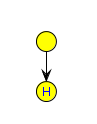
\includegraphics[width=50px]{img/hetero_homo.png}
	\centering
	\caption{El nodo con H contiene un secuente heterog'eneo. El otro nodo es homog'eneo.}
\end{figure}


\subsubsection{Ramas alternativas}

Para permitir documentar todas las acciones aplicadas as'i como la creaci'on de caminos de an'alisis alternativos introdujimos la noci'on de \textit{ramificaci'on alternativa}.
Las ramas alternativas representan la existencia de m'ultiples caminos en los que se subdivide el an'alisis para lograr un resultado. En la interfaz de usuario de Heterogenius este tipo de ramas se representa con lineas punteadas y su significado sem'antico es el de una disyunci'on \todomm{No entiendo esta frase. ¿Disyunción en qué sentido?}. Se corresponde con un camino alternativo en una demostraci'on.

\todomm{Siempre que puedas, no pongas figuras en la mitad de la página.}
\begin{figure}[htb]
	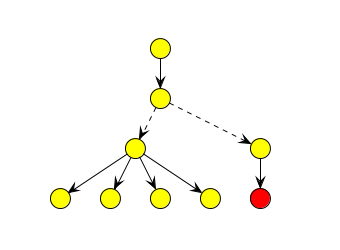
\includegraphics[width=180px]{img/ramas_alternativas_2.png}
	\centering
	\caption{La segunda rama alternativa presenta un contraejemplo. esto indica que existe un contraejemplo para el nodo del cual salen las ramas alternativas.}
        \label{alter1}
\end{figure}

Un nodo con hijos conectados por ramas alternativas se entiende que vale si \textit{\textbf{alguna}} de las ramas valen. Esto es diferente de la ramificaci'on normal (lineas continuas) que indica que el nodo padre vale si todos sus hijos valen.
\todomm{parrafo anterior: ¿Qué significa que un nodo “vale”? Reescribir el párrafo en términos de la “demostrabilidad” de la propiedad que se está analizando.}

Al aplicar una ramificaci'on alternativa a un nodo del 'arbol de an'alisis, el nodo es copiado y agregado como sus propios hijos \todomm{No me queda claro qué estás queriendo decir acá. ¿La copia del nodo es agregado como si fuera uno de sus hijos o se copia tanto el nodo como todos sus hijos?}. Esto nos permite trabajar sobre las copias del nodo original. Cuando es necesario tambi'en se puede agregar ramas alternativas durante un an'alisis.
 
La principal ventaja de usar caminos alternativos es la de poder documentar todo el an'alisis que se realiz'o y las decisiones tomadas, incluso las decisiones que no llevaron al cumplimiento del objetivo. Por otro lado tambi'en nos permite experimentar con diferentes formas de probar lo mismo.
En las Fig.~\ref{alter1} y \ref{alter2} se muestran ejemplos de estos usos.

\begin{figure}[bth]
	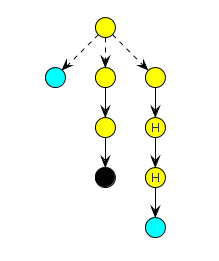
\includegraphics[width=100px]{img/ramas_alternativas.png}
	\centering
	\caption{Tres ramas alternativas: la primera y la 'ultima indican que no se encontr'o ning'un contraejemplo. La segunda rama muestra que se pudo demostrar que el secuente vale, por lo cu'al el secuente del nodo raiz tambi'en vale.}
        \label{alter2}
\end{figure}



\subsubsection{Nueva Clasificaci'on de Acciones}

\todomm{Esta explicación de cómo era el árbol de análisis de Heterogenius en la versión anterior debería estar en la sección 2.4 (Preliminares-Heterogenius)}

Como se ha mencionado, el elemento principal del proceso de demostración en Heterogenius es el 'arbol de an'alisis. All'i es donde se realizan todas las acciones y es donde se refleja el camino tomado para lograr una demostraci'on exitosa. Cada nodo del 'arbol representa un secuente en alg'un lenguaje soportado por Heterogenius. Las aristas se corresponden con las acciones aplicadas a cada secuente. Dependiendo del lenguaje en el que est'e el secuente se habilitan distintas acciones, pero en general se las puede dividir en tres categor'ias:

\begin{description}
\label{clasificacion}
\item[\textbf{reglas del c'alculo de secuentes}:] son acciones que transforman un secuente en otro. Algunas pueden producir múltiples secuentes (por ejemplo la acci'on \emph{Case}) creando varias ramas que tienen que ser demostradas para lograr un resultado en el nodo raiz.

\item[\textbf{traducciones}:] traducen un secuente de un lenguaje a otro. Dependiendo de la expresividad del lenguaje esta traducci'on puede preservar completamente la semántica o sólo parcialmente.

\item[\textbf{búsquedas de contraejemplos}:] implican el uso de herramientas externas para buscar contraejemplos para intentar validar el secuente donde se aplica la acci'on. 
Dependiendo del lenguaje del secuente y del poder de la herramienta seleccionada para realizar la búsqueda, estos procesos pueden verse como análisis parciales ya que podría ser imposible agotar todo el espacio de búsqueda. En tales contextos, una búsqueda infructuosa no brinda mayor información. Por el contrario, la existencia de un contraejemplo es prueba suficiente para saber que la rama en cuestión no podrá ser cerrada.
\end{description}

Si bien esta clasificaci'on serv'ia en la versi'on anterior, debi'o ser modificada para adaptarse a la nueva funcionalidad incluida durante el desarrollo de este trabajo y permitir una mayor flexibilidad a la hora de agregar otras herramientas en el futuro.
La nueva clasificaci'on propuesta se muestra a continuaci'on.

\begin{description}
\item[\textbf{Acciones de c'alculo de secuentes}:] esta categor'ia es ls misma que en la versi'on anterior. Comprende las acciones que permiten avanzar en el an'alisis aplicando reglas del c'alculo de secuentes.

\item[\textbf{Acciones de herramientas estructurales}:] son acciones que trabajan directamente sobre la estructura del 'arbol de an'alisis. Los traductores-$\rho$ forman parte de 'este grupo, asi como las nuevas acciones introducidas: \textit{traducci'on-$\rho$ de f'ormulas} y \textit{proyecci'on de f'ormulas}.

\item[\textbf{Acciones de herramientas automáticas}:] este grupo representa a las acciones para las que se usan herramientas autom'aticas como lo son los demostradores autom'aticos de teoremas y los buscadores de contraejemplos.
\end{description}

Esta clasificaci'on se reflej'o en la arquitectura de Heterogenius y permitir'a guiar las futuras extensiones y funcionalidades adicionales que se deseen implementar.
